% deck_programme.tex — the program in one picture: one shared prior, three
% swappable likelihood blocks.  Standalone TikZ; compile with tectonic.
\documentclass[tikz,border=8pt]{standalone}
\usepackage{amsmath,amssymb}
\usetikzlibrary{positioning,arrows.meta}

\definecolor{ink}{HTML}{1A1A1A}
\definecolor{muted}{HTML}{6B7280}
\definecolor{okblue}{HTML}{0072B2}
\definecolor{okamber}{HTML}{E69F00}
\definecolor{okverm}{HTML}{D55E00}
\definecolor{okgreen}{HTML}{009E73}

\begin{document}
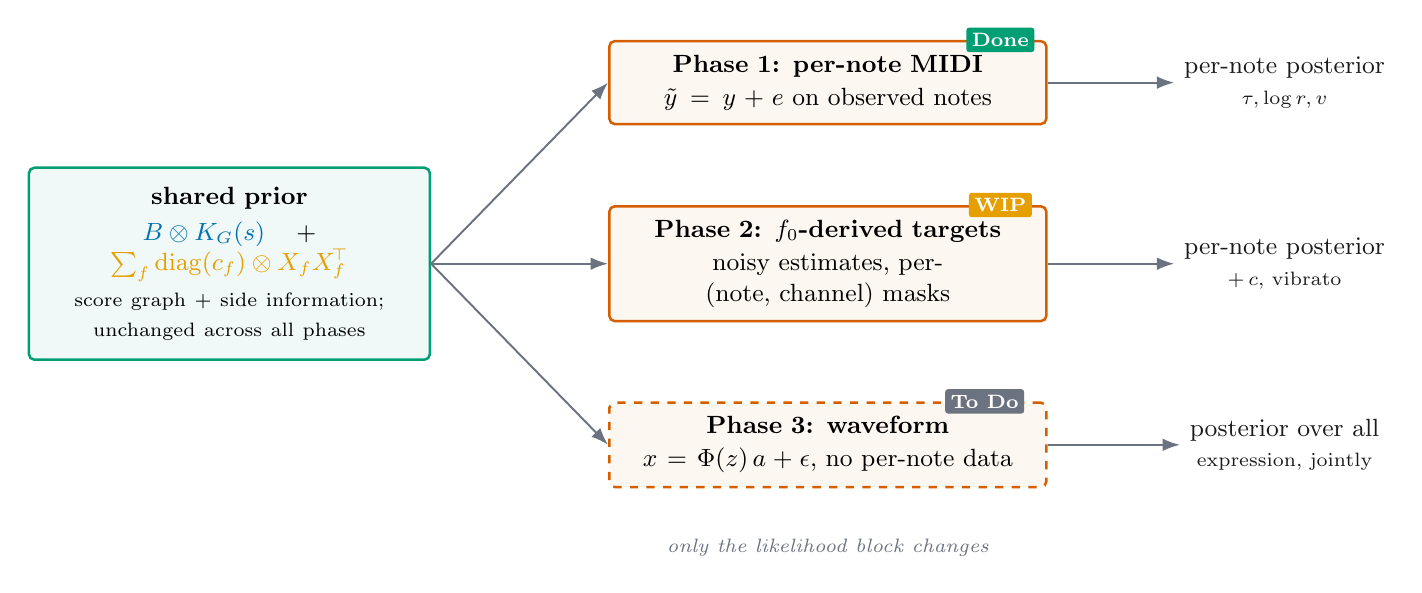
\begin{tikzpicture}[
  font=\small,
  prior/.style = {draw=okgreen, line width=0.9pt, rounded corners=2pt,
                  fill=okgreen!6, align=center, inner sep=7pt, text width=46mm},
  lik/.style   = {draw=okverm, line width=0.9pt, rounded corners=2pt,
                  fill=okverm!5, align=center, inner sep=5pt, text width=52mm},
  outp/.style  = {align=center, text=ink, font=\small},
  arr/.style   = {-{Latex[length=2.2mm,width=1.6mm]}, draw=muted, line width=0.7pt},
  tag/.style   = {font=\scriptsize\bfseries, text=white, fill=muted,
                  inner sep=2pt, rounded corners=1pt},
]

\node[prior] (prior) at (0,0)
  {\textbf{shared prior}\\[2pt]
   $\textcolor{okblue}{B \otimes K_G(s)} \;+\;
    \textcolor{okamber}{\sum_f \mathrm{diag}(c_f)\otimes X_f X_f^{\!\top}}$\\[3pt]
   {\scriptsize score graph + side information;\\ unchanged across all phases}};

\node[lik] (l1) at (7.6, 2.3)
  {\textbf{Phase 1: per-note MIDI}\\[1pt]
   $\tilde y = y + e$ on observed notes};
\node[lik] (l2) at (7.6, 0)
  {\textbf{Phase 2: $f_0$-derived targets}\\[1pt]
   noisy estimates, per-(note, channel) masks};
\node[lik, dashed] (l3) at (7.6, -2.3)
  {\textbf{Phase 3: waveform}\\[1pt]
   $x = \Phi(z)\,a + \epsilon$, no per-note data};

\node[tag, fill=okgreen] at ([xshift=-6mm, yshift=0mm]l1.east |- l1.north)  {Done};
\node[tag, fill=okamber] at ([xshift=-6mm]l2.east |- l2.north) {WIP};
\node[tag] at ([xshift=-8mm]l3.east |- l3.north) {To Do};

\node[outp] (o1) at (13.4, 2.3) {per-note posterior\\ {\scriptsize $\tau, \log r, v$}};
\node[outp] (o2) at (13.4, 0) {per-note posterior\\ {\scriptsize $+\,c$, vibrato}};
\node[outp] (o3) at (13.4, -2.3) {posterior over all\\ {\scriptsize expression, jointly}};

\draw[arr] (prior.east) -- (l1.west);
\draw[arr] (prior.east) -- (l2.west);
\draw[arr] (prior.east) -- (l3.west);
\draw[arr] (l1.east) -- (o1.west);
\draw[arr] (l2.east) -- (o2.west);
\draw[arr] (l3.east) -- (o3.west);

\node[font=\scriptsize\itshape, text=muted, align=center] at (7.6, -3.6)
  {only the likelihood block changes};

\end{tikzpicture}
\end{document}
